    \documentclass[dvipsnames, 10pt]{beamer}
    \usetheme{Madrid}
    \usefonttheme{professionalfonts}
    \usepackage{
        amsmath,
        amssymb,
        fouriernc, % fourier font w/ new century book
        fancyhdr, % page styling
        lastpage, % footer fanciness
        hyperref, % various links
        setspace, % line spacing
        amsthm, % newtheorem and proof environment
        mathtools, % \Aboxed for boxing inside aligns, among others
        float, % Allow [H] figure env alignment
        enumerate, % Allow custom enumerate numbering
        graphicx, % allow includegraphics with more filetypes
        wasysym, % \smiley!
        upgreek, % \upmu for \mum macro
        listings, % writing TrueType fonts and including code prettily
        tikz, % drawing things
        booktabs, % \bottomrule instead of hline apparently
        cancel % can cancel things out!
    }
    \usepackage[
        labelfont=bf, % caption names are labeled in bold
        font=scriptsize % smaller font for captions
    ]{caption}
    \usepackage[font=scriptsize]{subcaption} % subfigures

    \newcommand*{\scinot}[2]{#1\times10^{#2}}
    \newcommand*{\dotp}[2]{\left<#1\,\middle|\,#2\right>}
    \newcommand*{\rd}[2]{\frac{\mathrm{d}#1}{\mathrm{d}#2}}
    \newcommand*{\pd}[2]{\frac{\partial#1}{\partial#2}}
    \newcommand*{\rtd}[2]{\frac{\mathrm{d}^2#1}{\mathrm{d}#2^2}}
    \newcommand*{\ptd}[2]{\frac{\partial^2 #1}{\partial#2^2}}
    \newcommand*{\md}[2]{\frac{\mathrm{D}#1}{\mathrm{D}#2}}
    \newcommand*{\pvec}[1]{\vec{#1}^{\,\prime}}
    \newcommand*{\svec}[1]{\vec{#1}\;\!}
    \newcommand*{\bm}[1]{\boldsymbol{\mathbf{#1}}}
    \newcommand*{\ang}[0]{\;\text{\AA}}
    \newcommand*{\mum}[0]{\\;upmu \mathrm{m}}
    \newcommand*{\at}[1]{\left.#1\right|}

    \let\Re\undefined
    \let\Im\undefined
    \DeclareMathOperator{\Res}{Res}
    \DeclareMathOperator{\Re}{Re}
    \DeclareMathOperator{\Im}{Im}
    \DeclareMathOperator{\Log}{Log}
    \DeclareMathOperator{\Arg}{Arg}
    \DeclareMathOperator{\Tr}{Tr}
    \DeclareMathOperator{\E}{E}
    \DeclareMathOperator{\Var}{Var}
    \DeclareMathOperator*{\argmin}{argmin}
    \DeclareMathOperator*{\argmax}{argmax}
    \DeclareMathOperator{\sgn}{sgn}
    \DeclareMathOperator{\diag}{diag\;}

    \DeclarePairedDelimiter\bra{\langle}{\rvert}
    \DeclarePairedDelimiter\ket{\lvert}{\rangle}
    \DeclarePairedDelimiter\abs{\lvert}{\rvert}
    \DeclarePairedDelimiter\ev{\langle}{\rangle}
    \DeclarePairedDelimiter\p{\lparen}{\rparen}
    \DeclarePairedDelimiter\s{\lbrack}{\rbrack}
    \DeclarePairedDelimiter\z{\lbrace}{\rbrace}

    % \everymath{\displaystyle} % biggify limits of inline sums and integrals
    \tikzstyle{circ} % usage: \node[circ, placement] (label) {text};
        = [draw, circle, fill=white, node distance=3cm, minimum height=2em]
    \definecolor{commentgreen}{rgb}{0,0.6,0}
    \lstset{
        basicstyle=\ttfamily\footnotesize,
        frame=single,
        numbers=left,
        showstringspaces=false,
        keywordstyle=\color{blue},
        stringstyle=\color{purple},
        commentstyle=\color{commentgreen},
        morecomment=[l][\color{magenta}]{\#}
    }

\begin{document}

\title[IGWs \& Mean Flow Steepening]{
Mean Flow Steepening in Internal Gravity Wave Breaking}
\subtitle{Group Meeting Presentation}
\author{Yubo Su}
\date{Nov 30, 2018}

\maketitle

\begin{frame}
    \frametitle{Background}
    \framesubtitle{Problem Setup}

    \begin{itemize}
        \item 2D plane parallel atmosphere, continuous train IGW from below.

        \item Equations to filter sound waves (actually surprisingly
            contentious):
            \begin{align}
                \vec{\nabla} \cdot \vec{u} &= 0,\\
                \pd{\rho_1}{t} -{}& \frac{u_{1z} \rho_0}{H}
                    + \vec{u} \cdot \vec{\nabla}\rho_1\nonumber\\
                    &= \s*{-\Gamma(z) + \mathfrak{D}}\rho_1
                    + \z*{Fe^{-\frac{(z - z_0)^2}{2\sigma^2}} \cos\p*{k_xx -
                    \omega t}},\\
                \pd{\vec{u}}{t} +{}& \p*{\vec{u} \cdot \vec{\nabla}}\vec{u}
                    + \frac{\vec{\nabla}P_1}{\rho_0}
                    + \frac{\rho_1 \vec{g}}{\rho_0}
                    - \frac{\vec{\nabla}P_1}{\rho_0}\rho_1\nonumber\\
                    &= \s*{-\Gamma(z) + \mathfrak{D}}\vec{u}
            \end{align}

        \begin{itemize}
            \item $\Gamma(z) \propto 2 + \tanh\p*{\frac{z - z_H}{w}} +
                \tanh\p*{\frac{z_b - z}{w}}, \mathfrak{D} \sim \nabla^{k}$.
                ($[]$ numerical, $\z*{}$ forcing).

            \item If $\rd{\ln \rho_0}{z} = H$ scale height $\gg$ domain of
                simulation, can use $\rho_0(z) = \rho_0$, \emph{Boussinesq
                approximation}. Else, $\sim$ \emph{anelastic}.
        \end{itemize}
    \end{itemize}
\end{frame}

\begin{frame}
    \frametitle{Background}
    \framesubtitle{Theory}

    \begin{itemize}
        \item Perturbation $\p*{\vec{u}, \rho_1, P_1}$ carries average
            horizontal momentum flux $\ev*{F_{p, x}}_x = \ev*{\rho u_x u_z}$.

        \item Induces mean flow
            \begin{equation}
                 \ev*{u_x}_x \equiv \bar{U}_x(z) \neq 0
                    = \frac{\ev*{u_xu_z}_x}{c_{g, z}}.
            \end{equation}

        \item Critical layer (equivalent to corotation resonance in other
            systems): where Doppler-shifted frequency (in fluid rest frame)
            $\omega \Rightarrow \omega - k_x\bar{U}_x = 0$.

        \item Since $\vec{u} \propto e^{z/2H}$, so $\bar{U}_x \propto e^{z/H}$,
            $\exists \,z_c\!: \omega - k_x\bar{U}_x(z_c) = 0$.
    \end{itemize}
\end{frame}

\begin{frame}
    \frametitle{Background}
    \framesubtitle{Hypothesis}


    \begin{itemize}
        \item Since critical layers almost always induce full absorption
            (recall, $\propto \exp\s*{-\pi \sqrt{\mathrm{Ri}^2 -
            \frac{1}{4}}}, \mathrm{Ri} = \frac{N}{\bar{U}_x'}$),
            hypothesis:

            \begin{itemize}
                \item $\vec{u}_1$ is excited, induces $\bar{U}_x$ mean flow.

                \item Once $\bar{U}_x$ satisfies critical layer criterion,
                    $F_{p, x}$ is fully absorbed.

                \item Horizontal momentum goes into spinning up more fluid up to
                    $\bar{U}_{x, crit} = \frac{\omega}{k_x}$.

                \item Thus, critical layer should propagate down.
            \end{itemize}

        \item Exactly \emph{quasi-biennial oscillation} theory (Lindzen 1980,
            1982), assume critical layer breaks down eventually.

        \item Already different from naive ``goes nonlinear and deposits
            locally'' theory!
    \end{itemize}
\end{frame}

\begin{frame}
    \frametitle{Simulations}
    \framesubtitle{Large Anelastic, Low-Amplitude}

    \begin{itemize}
        \item Permit $z \in [0H, 10H]$, full $\rho_0 \propto e^{-z/H}$, allow
            $\vec{u} \propto e^{z/2H}$ to source growing mean flow.

        \item Low-Amplitude ($k_z\xi_z \ll 1$ everywhere). Orange = analytical
            solution.
    \end{itemize}
    \begin{figure}[t]
        \centering
        \hspace*{-19mm}%
        \begin{subfigure}{0.55\textwidth}
            \centering
            % linear_1/t_018.png
            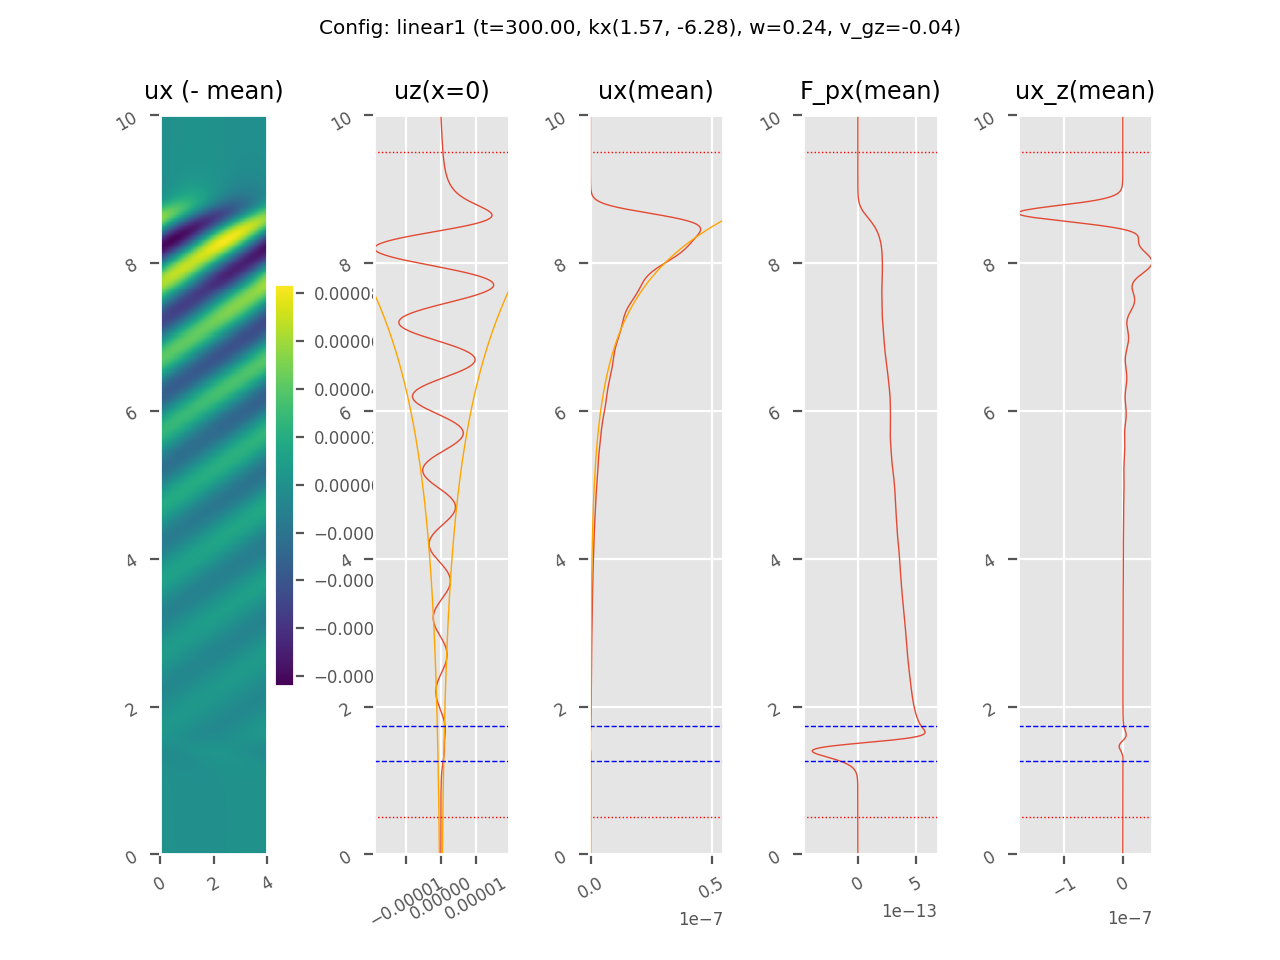
\includegraphics[width=\textwidth]{lin_early.png}
            \caption{Early Low-A}
        \end{subfigure}
        \begin{subfigure}{0.55\textwidth}
            \centering
            % linear_1/t_049.png
            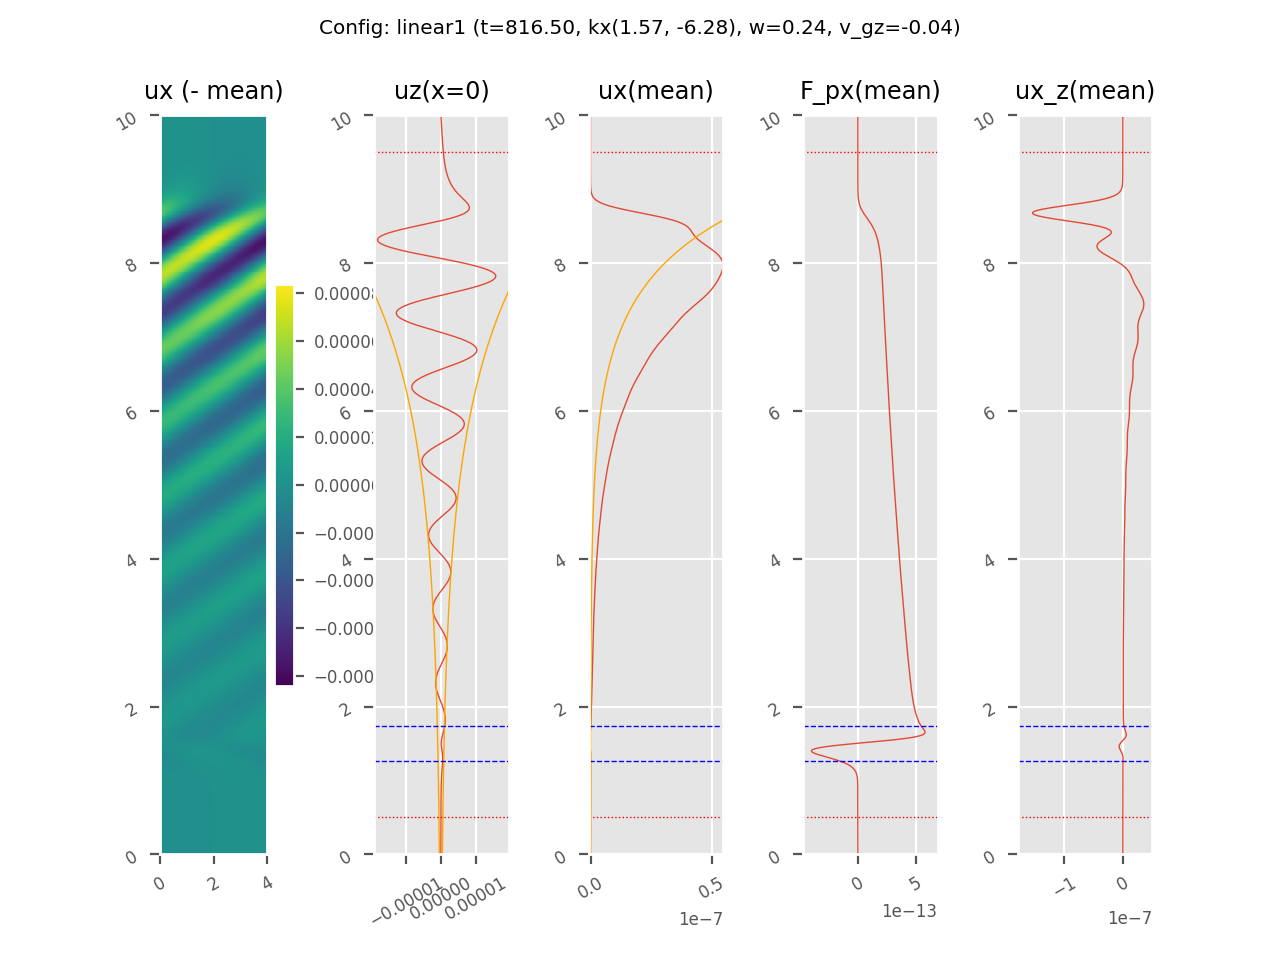
\includegraphics[width=\textwidth]{lin_late.png}
            \caption{Later Low-A}
        \end{subfigure}
        \hspace*{-19mm}%
    \end{figure}
\end{frame}

\begin{frame}
    \frametitle{Simulations}
    \framesubtitle{Large Anelastic, Low-Amplitude}

    \begin{figure}[t]
        \centering
        % linear0/t_045.png
        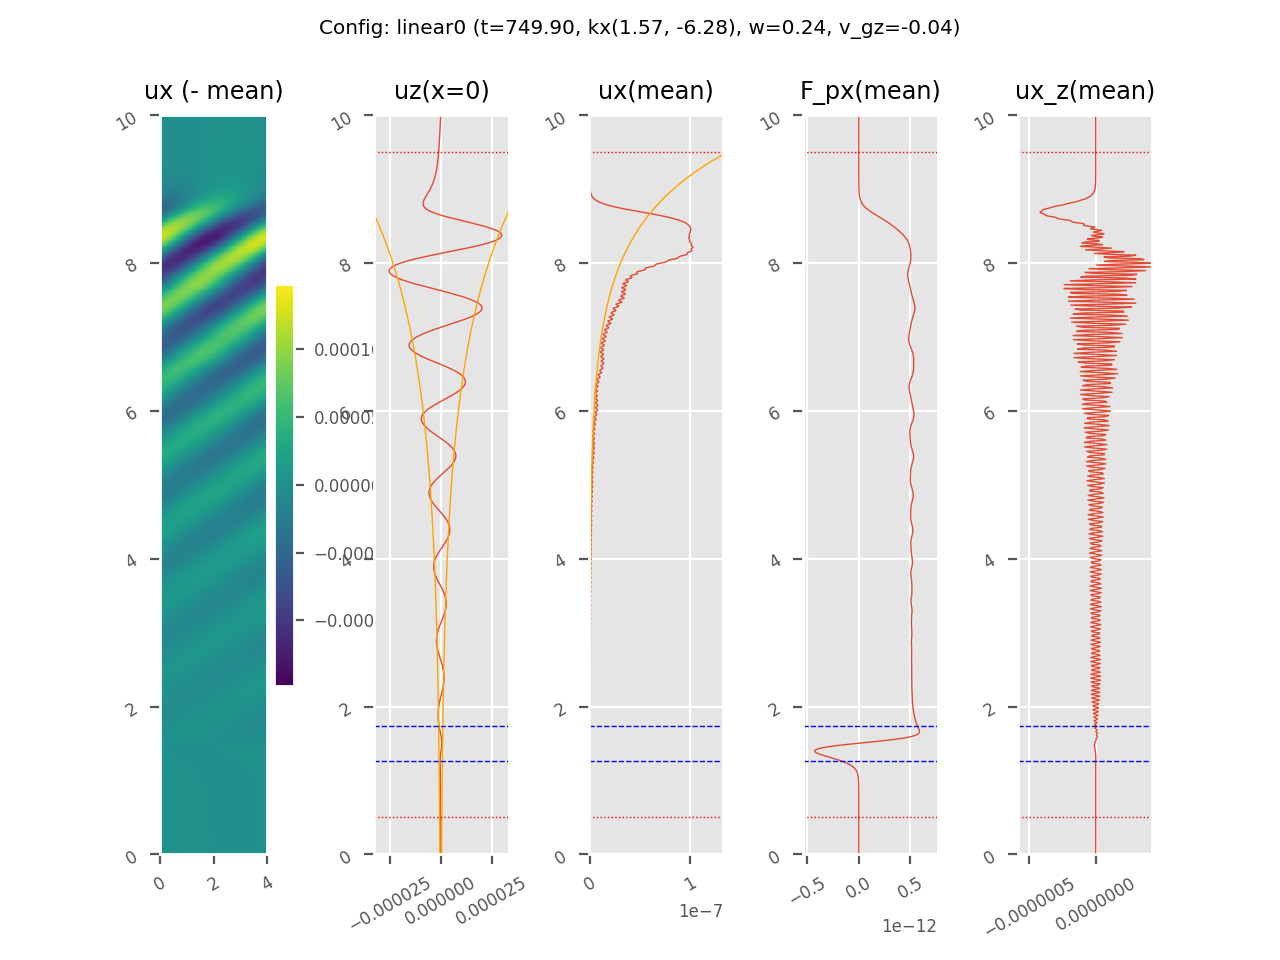
\includegraphics[width=0.55\textwidth]{lin_nonu.png}
        \caption{Low-Amplitude, nearly zero viscosity.}
    \end{figure}
\end{frame}

\begin{frame}
    \frametitle{Simulations}
    \framesubtitle{Large Anelastic, High-Amplitude}

    \begin{itemize}
        \item Note steepening region ($N = 1$, so $\pd{\bar{U}_x}{z} =
            \mathrm{Ri}^{-1}$).
    \end{itemize}

    \begin{figure}[t]
        \centering
        \hspace*{-19mm}%
        \begin{subfigure}{0.53\textwidth}
            \centering
            % nl1/t_029.png
            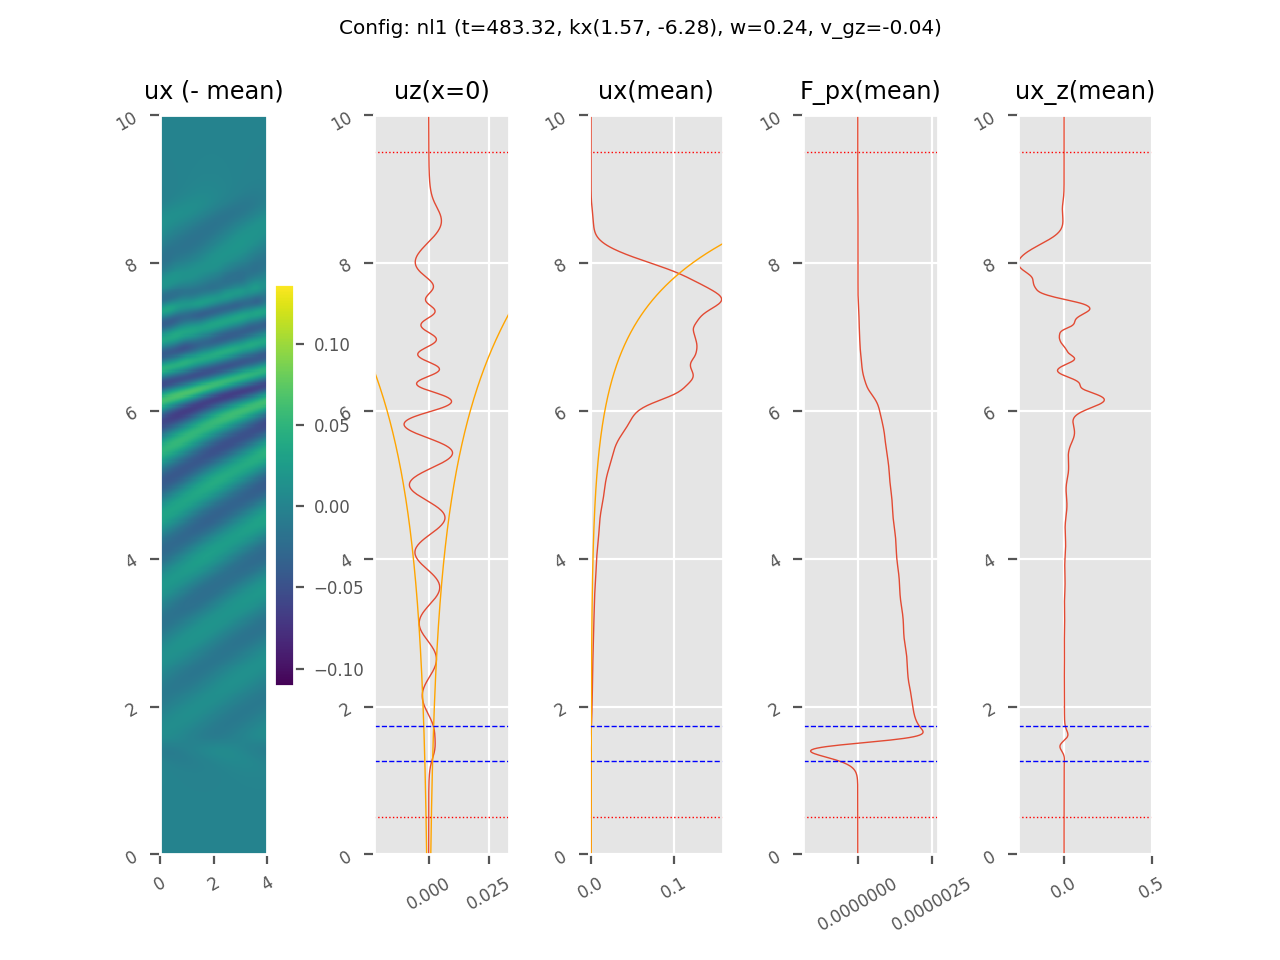
\includegraphics[width=\textwidth]{nl_low_1.png}
            \caption{Lower-res.}
        \end{subfigure}
        \begin{subfigure}{0.53\textwidth}
            \centering
            % nl_full/t_029.png
            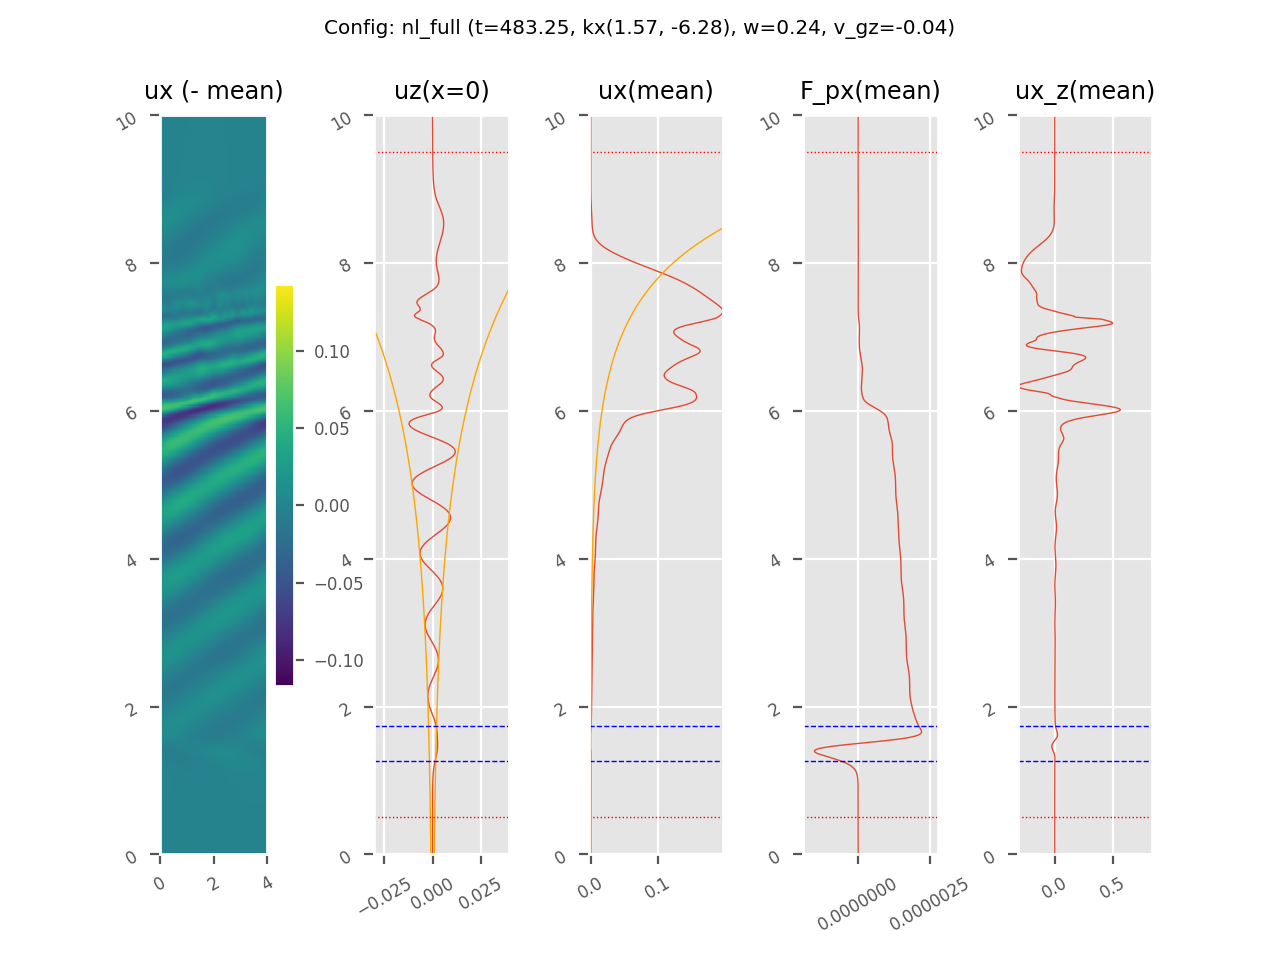
\includegraphics[width=\textwidth]{nl_full_1.png}
            \caption{Double $N_z$.}
        \end{subfigure}
        \hspace*{-19mm}%
    \end{figure}
\end{frame}

\begin{frame}
    \frametitle{Simulations}
    \framesubtitle{Large Anelastic, High-Amplitude}

    \begin{itemize}
        \item Later
    \end{itemize}

    \begin{figure}[t]
        \centering
        \hspace*{-19mm}%
        \begin{subfigure}{0.53\textwidth}
            \centering
            % nl1/t_049.png
            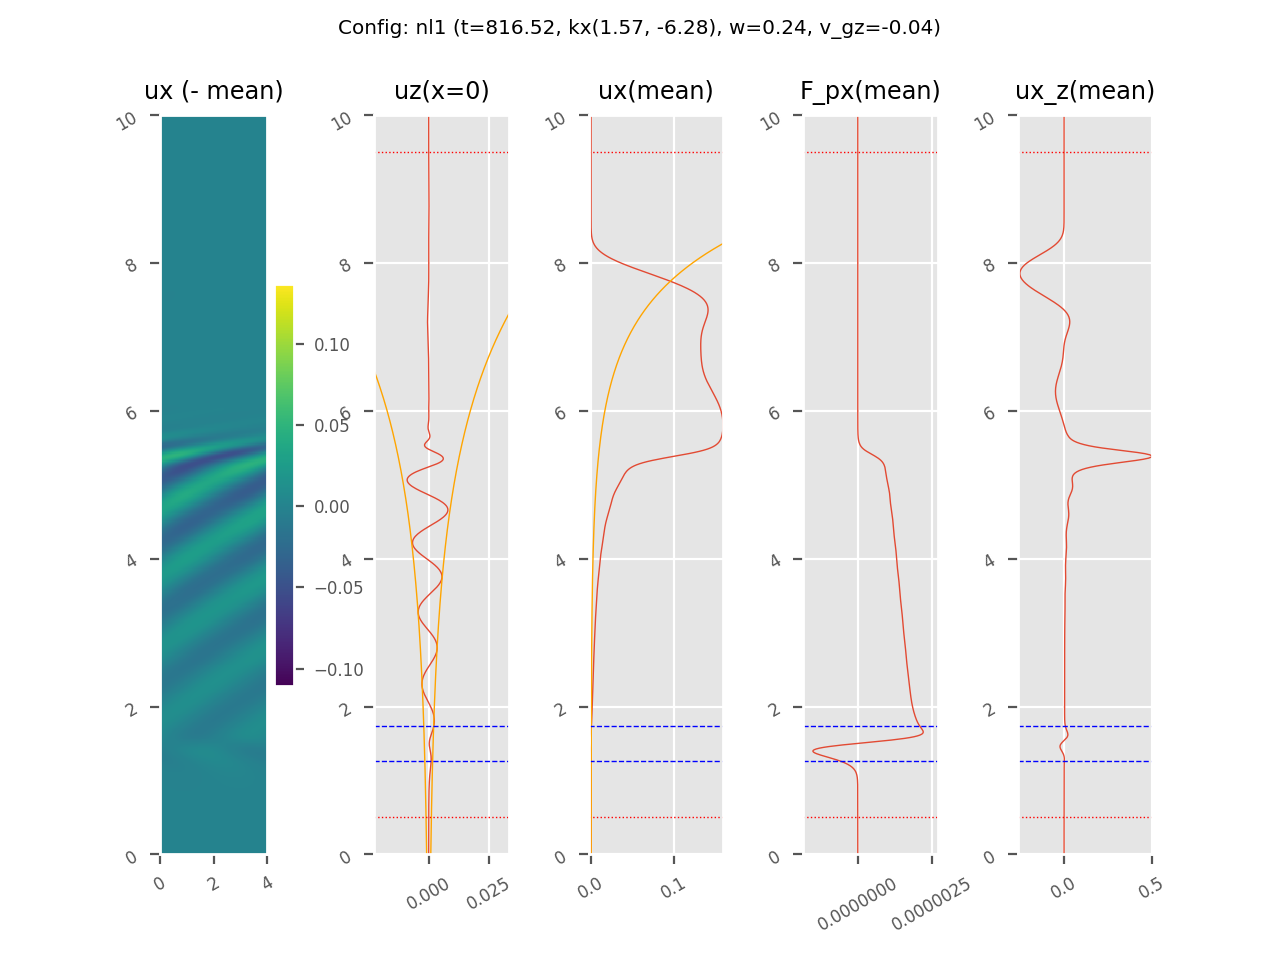
\includegraphics[width=\textwidth]{nl_low_2.png}
            \caption{Lower-res.}
        \end{subfigure}
        \begin{subfigure}{0.53\textwidth}
            \centering
            % nl_full/t_049.png
            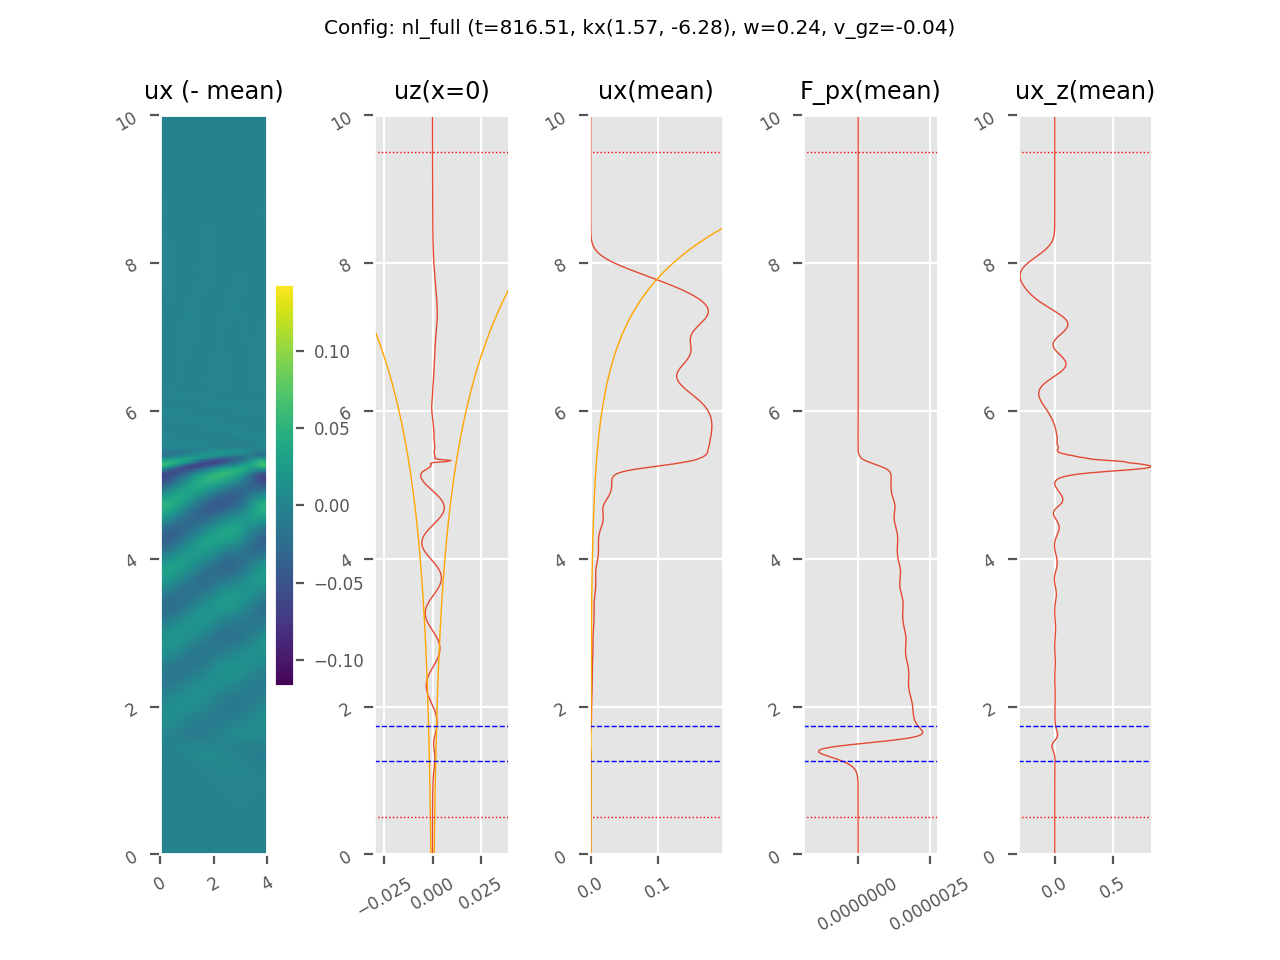
\includegraphics[width=\textwidth]{nl_full_2.png}
            \caption{Double $N_z$.}
        \end{subfigure}
        \hspace*{-19mm}%
    \end{figure}
\end{frame}

\begin{frame}
    \frametitle{Simulations}
    \framesubtitle{Large Anelastic, Comments}

    \begin{itemize}
        \item While damping layers pump up $\bar{U}_x$, ran on higher amplitude,
            damping layer is not chief cause of $\bar{U}_x$ critical layer
            behavior. % nl2.png, nl2/t_018.png

        \item Would expect reflections, but \emph{viscously limited}?
            \begin{itemize}
                \item Indeed, $\mathrm{Ri}^{-1} \sim \abs*{\vec{k}}d$ where $d$
                    is the width of the spinup layer, then $\nu \rho_0
                    \frac{\bar{U}_{x, c}}{d^2} \sim \frac{F_{p, x}}{d}$.
            \end{itemize}

        \item Matching $F_{p, x} = \ev*{\rho_0 u_x u_z}$ with spinning up mass
            $F_{p, x} = u_{front} \rho_0 \bar{U}_{x, crit}$ lets us predict
            $u_{front}$, next page.
    \end{itemize}
\end{frame}

\begin{frame}
    \frametitle{Simulations}
    \framesubtitle{Large Anelastic, Predicting $u_{front}$}

    \begin{itemize}
        \item Front position is $z_f = \argmax_z \rd{\bar{U}_x}{z}$, while
            $F_{p, x} = 2F_{p, x}(z_f)$ ($\sim$ halfway in front).

        \item Predicts $u_{front} = \frac{F_{p, x}}{\rho_0(z) \bar{U}_{x, c}}
            \approx \scinot{2.2}{-3}NH$ (using $z \approx 5.5H$), or $2H/3$ in
            $300N$. Pretty close, seems to imply perfect absorption.
    \end{itemize}
    \begin{figure}[t]
        \centering
        \hspace*{-19mm}%
        \begin{subfigure}{0.53\textwidth}
            \centering
            % nl1/t_049.png
            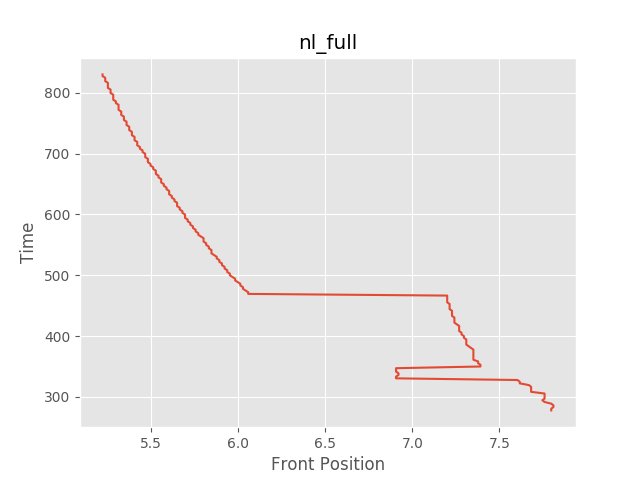
\includegraphics[width=\textwidth]{front_nl_full.png}
            \caption{Front Position. Slight exponential.}
        \end{subfigure}
        \begin{subfigure}{0.53\textwidth}
            \centering
            % nl_full/t_049.png
            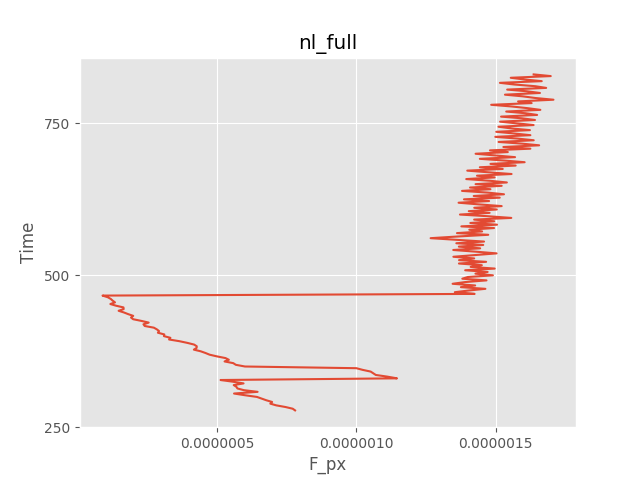
\includegraphics[width=\textwidth]{fluxes_nl_full.png}
            \caption{$F_{p, x} = \ev*{\rho_0 u_x u_z}_x$.}
        \end{subfigure}
        \hspace*{-19mm}%
    \end{figure}
\end{frame}

\begin{frame}
    \frametitle{Simulations}
    \framesubtitle{Local Boussinesq}

    \begin{itemize}
        \item Go to Boussinesq, ``zoom in.'' Use $\mathfrak{D} = \nabla^6$
            regularization. Set up initial mean flow $\bar{U}_x(z)$ such that
            $\max_z \bar{U}_x(z) = \bar{U}_{x, c}$.

        \item Reflection indeed develops!
    \end{itemize}

    \begin{figure}[t]
        \centering
        \hspace*{-19mm}%
        \begin{subfigure}{0.55\textwidth}
            \centering
            % vstrat/t_000.png
            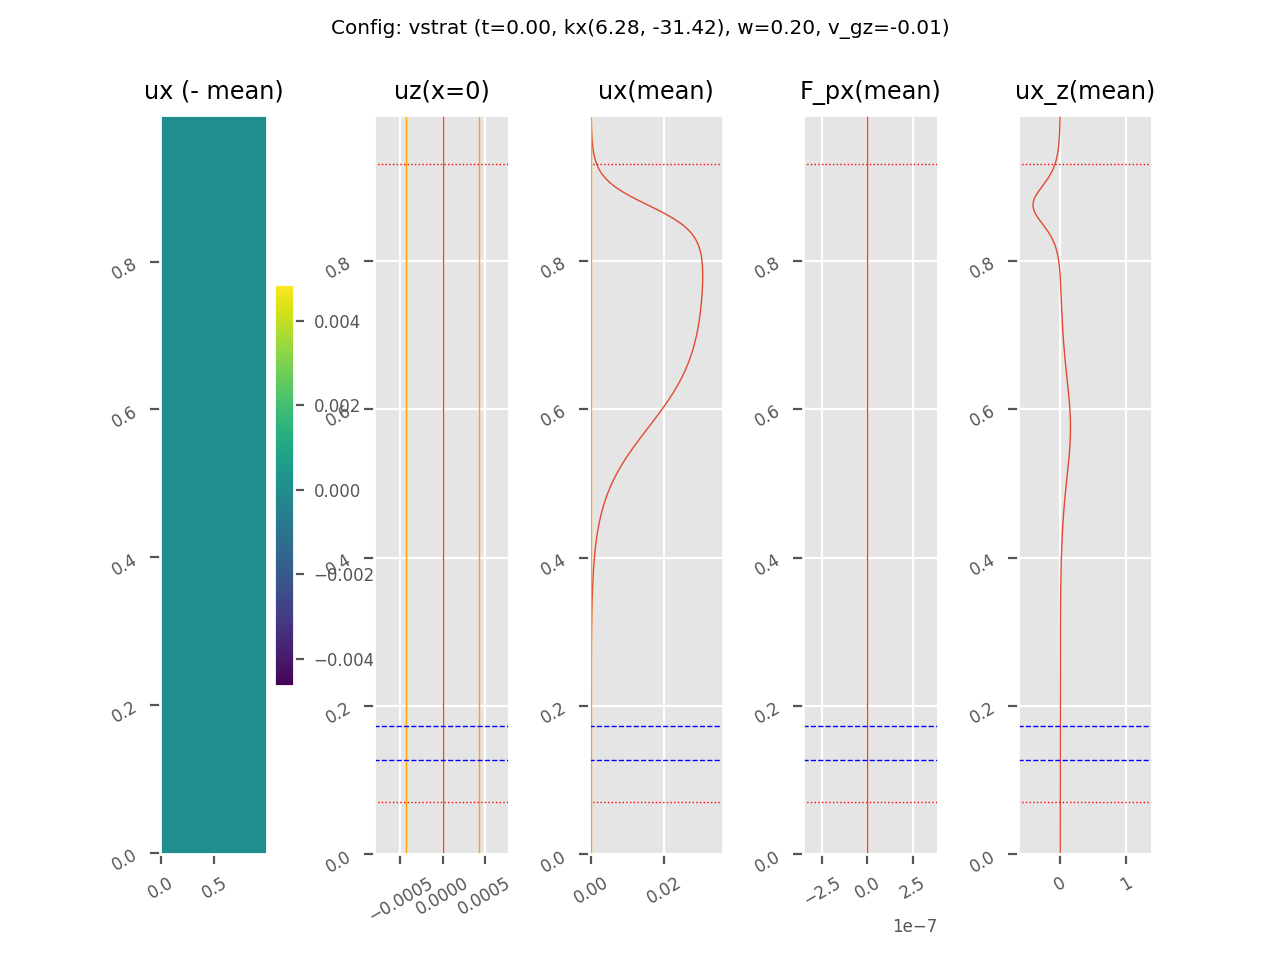
\includegraphics[width=\textwidth]{vstrat_0.png}
        \end{subfigure}
        \begin{subfigure}{0.55\textwidth}
            \centering
            % vstrat/t_010.png
            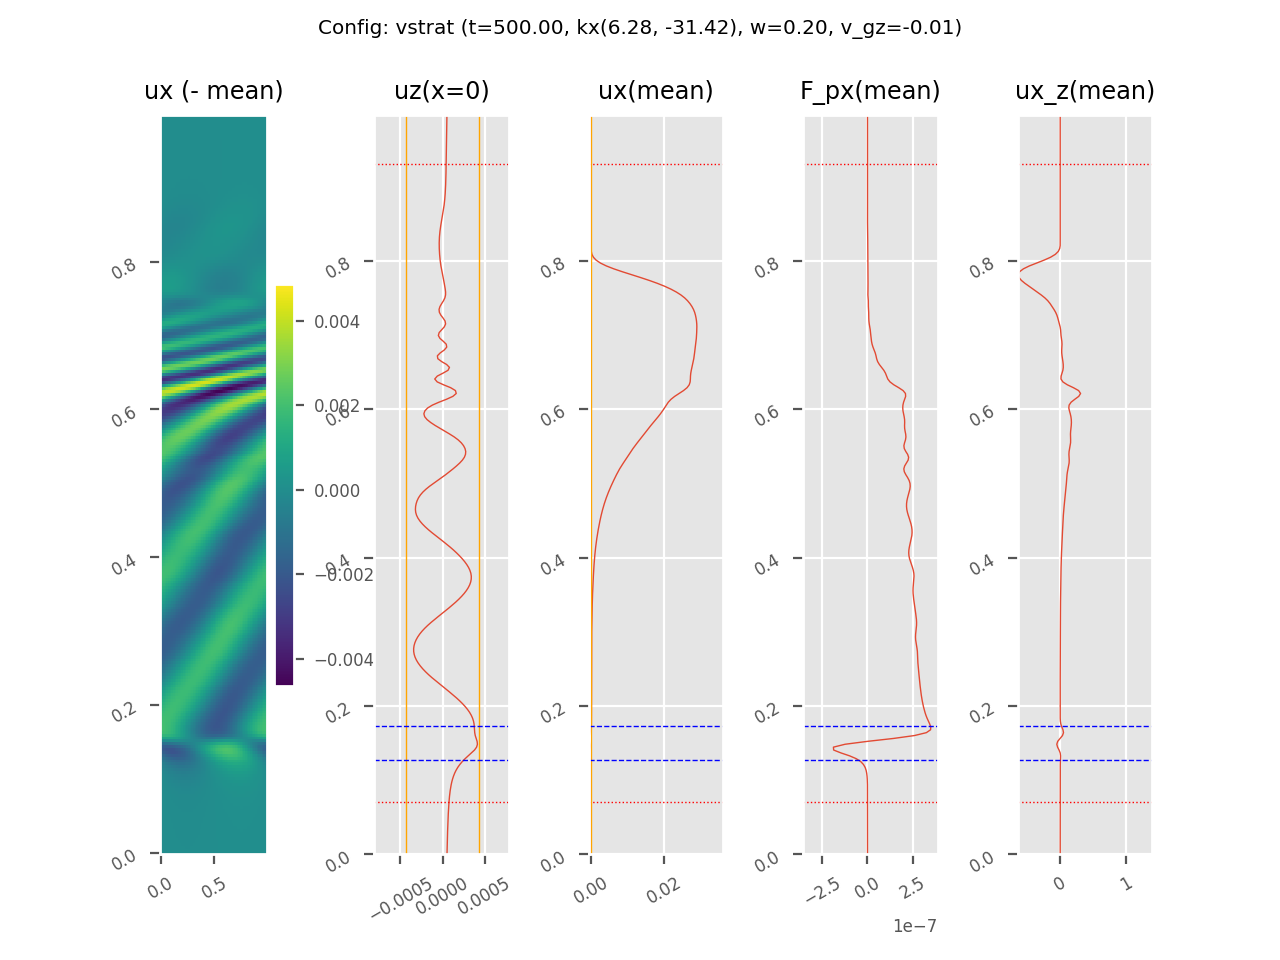
\includegraphics[width=\textwidth]{vstrat_1.png}
        \end{subfigure}
        \hspace*{-19mm}%
    \end{figure}
\end{frame}

\begin{frame}
    \frametitle{Simulations}
    \framesubtitle{Local Boussinesq}
    \begin{itemize}
        \item Expect Kelvin-Helmholtz instability to develop; resolution-limit?
            Tried with random noise, no qualitative difference.

        \item Not viscosity-limited: $\nu^{(6)} \rho_0
            \frac{\bar{U}_{x, c}}{d^6} \ll \frac{F_{p, x}}{d}$!
    \end{itemize}

    \begin{figure}[t]
        \centering
        \hspace*{-19mm}%
        \begin{subfigure}{0.55\textwidth}
            \centering
            % vstrat/t_040.png
            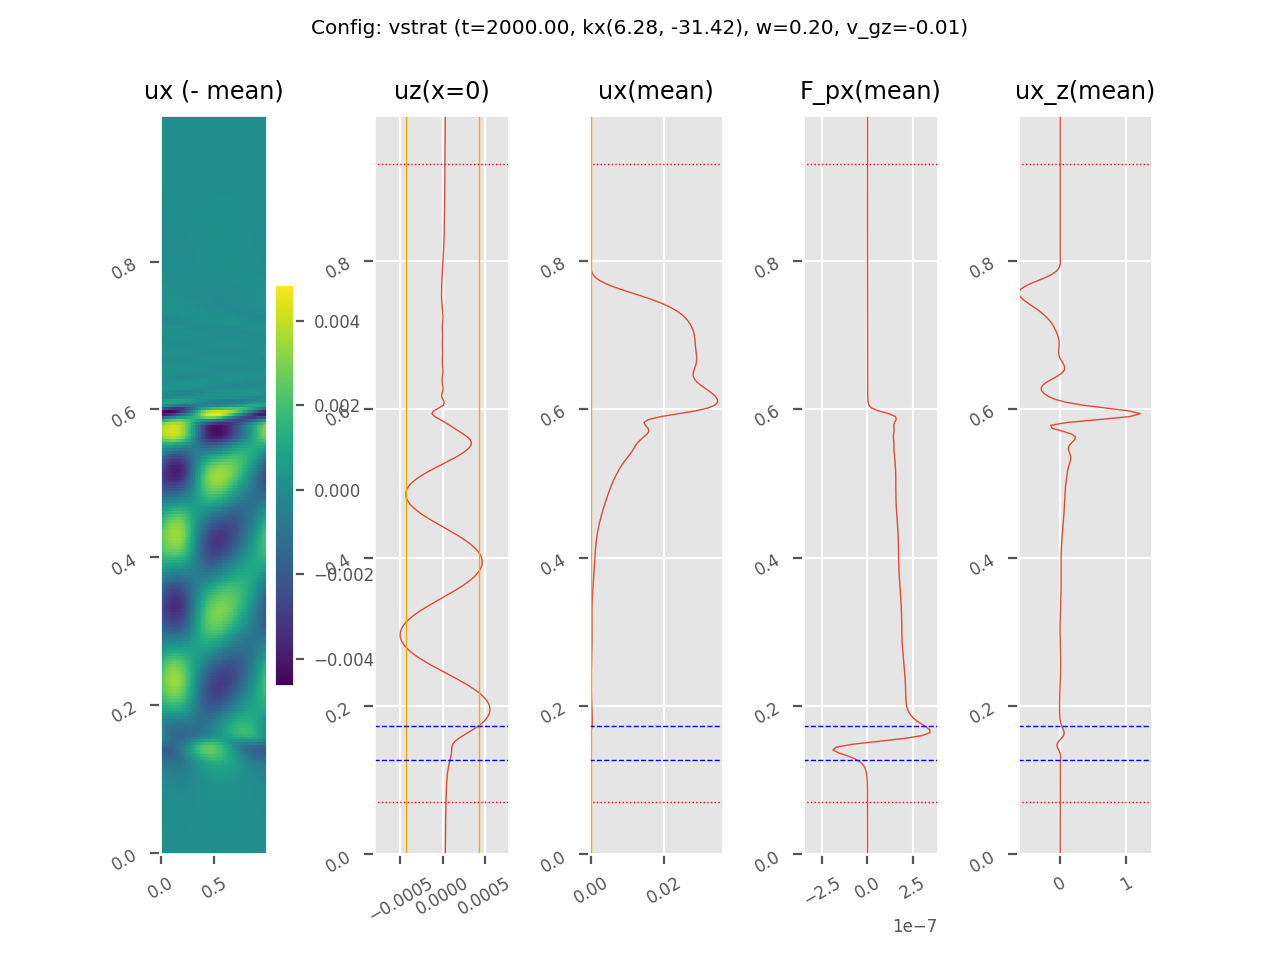
\includegraphics[width=\textwidth]{vstrat_2.png}
        \end{subfigure}
        \begin{subfigure}{0.55\textwidth}
            \centering
            % vstrat/t_065.png
            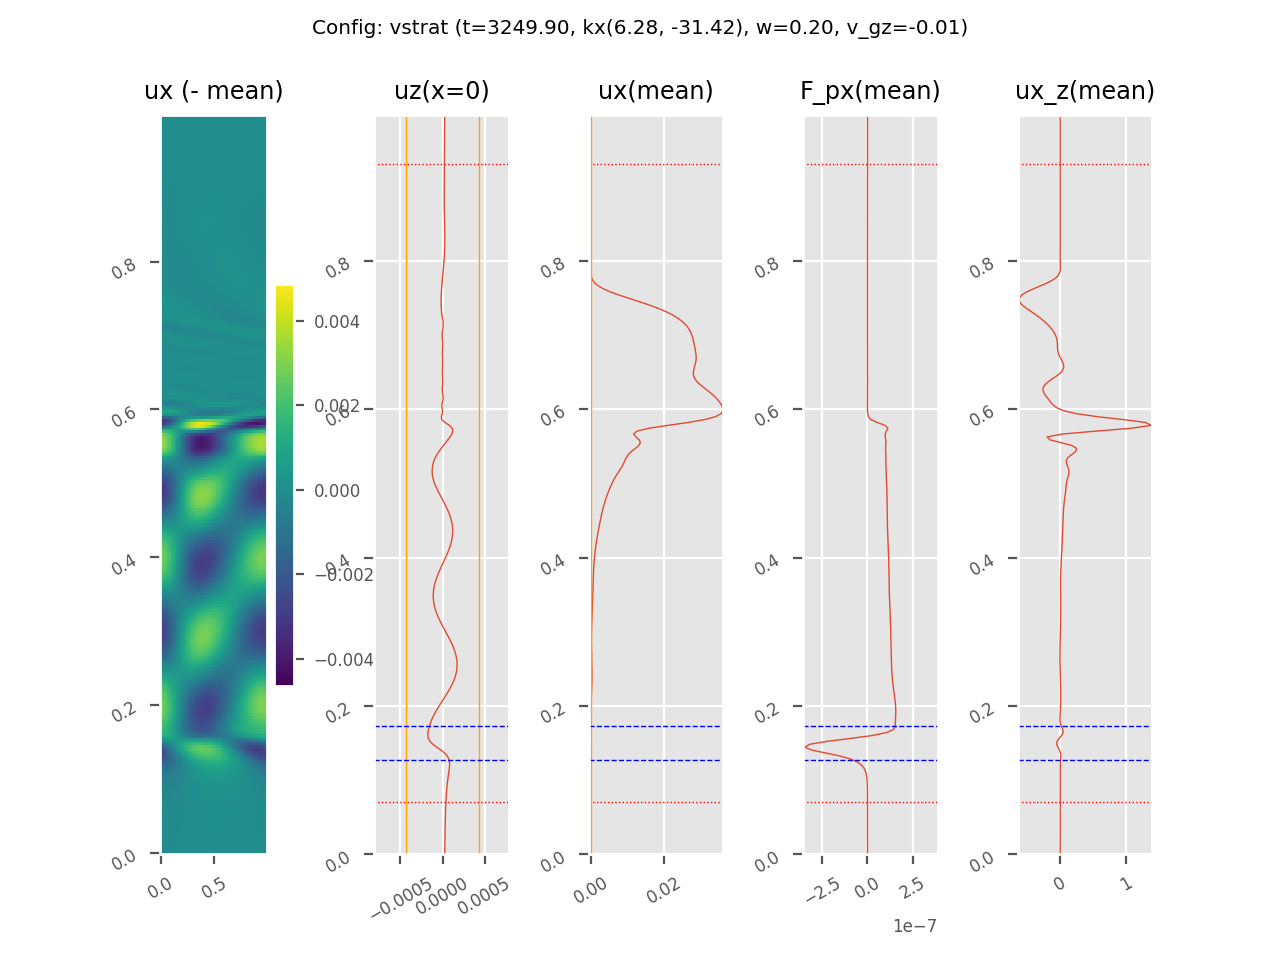
\includegraphics[width=\textwidth]{vstrat_3.png}
        \end{subfigure}
        \hspace*{-19mm}%
    \end{figure}
\end{frame}

\begin{frame}
    \frametitle{Simulations}
    \framesubtitle{Comparing $u_{front}$}

    \begin{itemize}
        \item Same as for anelastic, but predicts
            $u_{front} \approx \frac{\scinot{4.5}{-7}}{\rho_0 \bar{U}_{x, c}}
            \approx \scinot{1.4}{-5}HN$ or $0.014H$ in $1000N$. $t \in [1000,
            2000]$ accurate, $t \in [2000, 3000]$ less so.

        \item No front slowdown is expected since $\rho_0$ is constant in space,
            but is observed; could be explained by increasing reflectivity.
    \end{itemize}
    \begin{figure}[t]
        \centering
        \hspace*{-19mm}%
        \begin{subfigure}{0.53\textwidth}
            \centering
            % nl1/t_049.png
            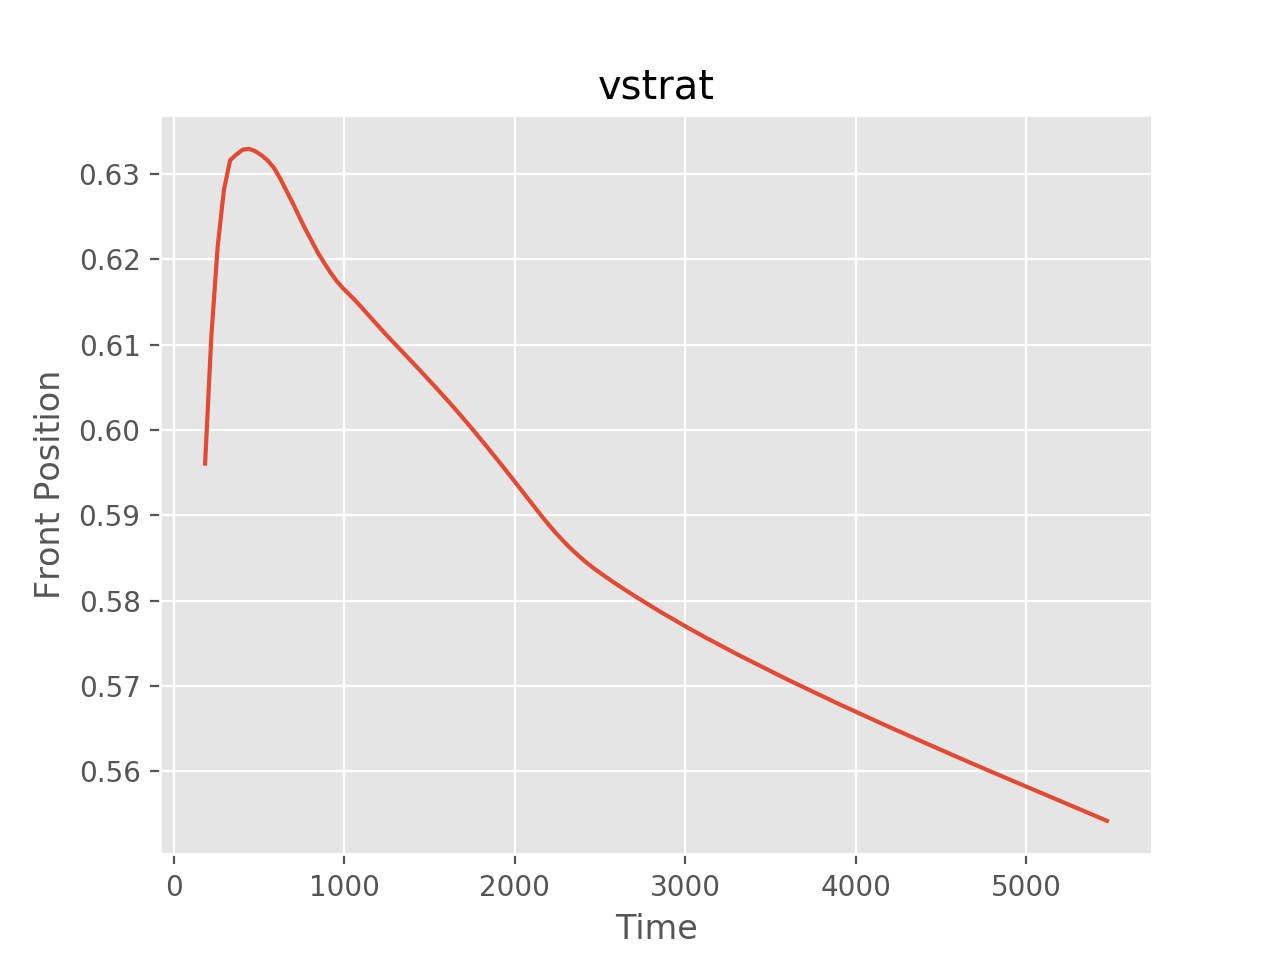
\includegraphics[width=\textwidth]{front_vstrat.png}
            \caption{Front Position. Slowing down.}
        \end{subfigure}
        \begin{subfigure}{0.53\textwidth}
            \centering
            % nl_full/t_049.png
            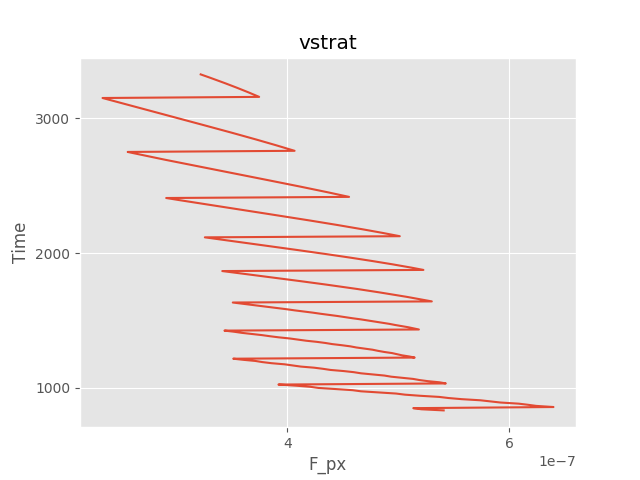
\includegraphics[width=\textwidth]{fluxes_vstrat.png}
            \caption{$F_{p, x}$.}
        \end{subfigure}
        \hspace*{-19mm}%
    \end{figure}
\end{frame}

\end{document}

